\subsection{Entity-Relationship Schema}

\begin{center}
	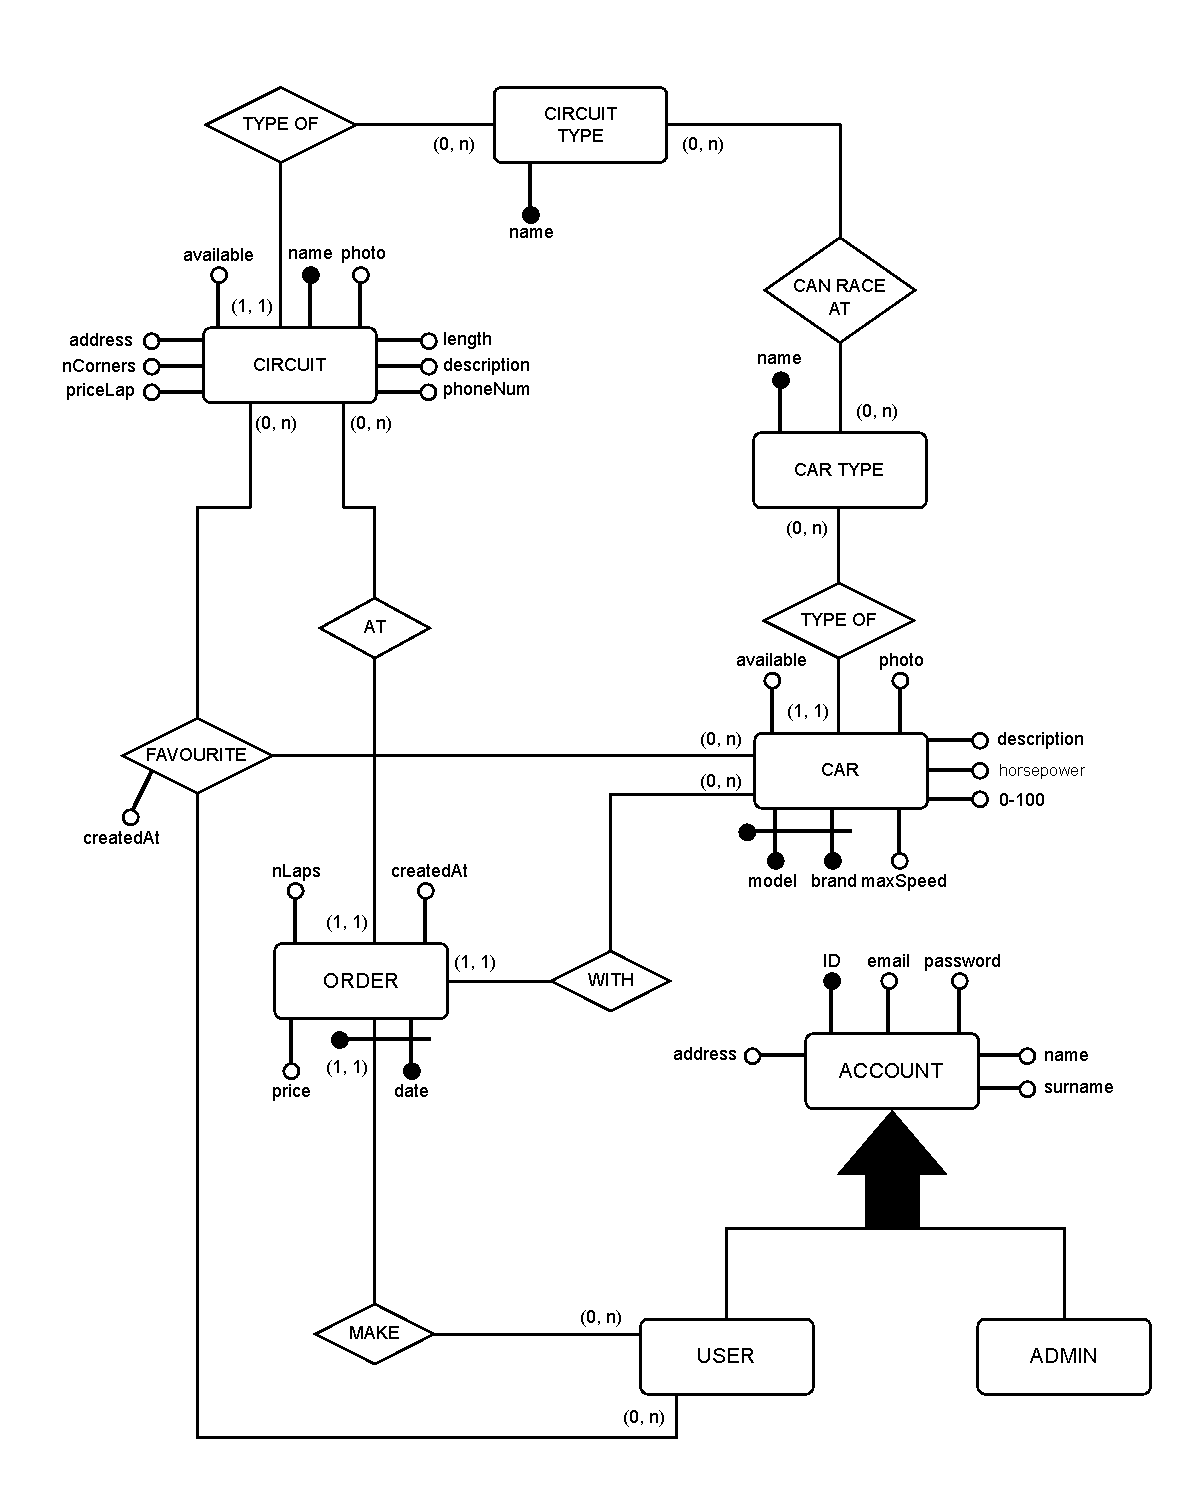
\includegraphics[scale=0.55]{ERSchema.pdf}
	\captionof{figure}{ER schema of WACAR}
	\label{ERSchema}
\end{center}

The ER schema contains the following entities:
\begin{itemize}
	\item \textbf{account}:the account contains both the account for the users of the web app and the admin that manages the contents of the tables. It has an id (type INTGER) that increments at every user added. Then, it has the email and password used for signing in (both are type CHARACTER VARYING), the name (type CHARACTER VARYING) and surname (type CHARACTER VARYING) and the address (type TEXT). Finally, it has the attribute type that is an enumerator and can assume value "USER" or "ADMIN" for specifying the type of the account. An account have a 0-N relationship with entity \textit{order}, so that it can make more than one order. Finally, an account can also add a pair \textit{car-circuit} in a bookmarks list represented by the relationship \textit{favourite}.
	\item \textbf{car}: it represents the entity for the car users car drive. Its primary key is composed by the brand and the model of a car (both type CHARACTER VARYING), some data are about the performance of the car (horsepower, 0-100 and maxSpeed, the first one is type INTEGER and the others CHARACTER VARYING) and for general spacifications there is the description (type TEXT). Finally, it has a foreign key for the type of the car (e.g. 'supercar').
	\item \textbf{circuit}: this entity represents the circuit in which users can race. It it identified by its name (type CHARACTER VARYING). Then, it contains the address (type TEXT), the price for doing a lap (type INTEGER) and some characteristics such as the length (type CHARACTER VARYING), the number of corners (type INTEGER) and a general description (type TEXT). Finally it has a foreign key for the type of circuit (e.g 'tarmac'). 
	\item \textbf{circuitType} and \textbf{carType}: the first entity contains the name (type CHARACTER VARYING) of the type of a circuit, while the second entity contains the name (type CHARACTER VARYING) of the type of a car. Those entities are related to each other by the 0-N \textit{can race at} relationship. This relationship saves the suitability between a type of circuit and a type of car: for example, if a pair circuitType-carType is composed by 'tarmac'-'supercar', then this means that a supercar can race on that circuit. Otherwise, if the pair 'rallycross'-'supercar' is not present, then the supercar cannot race on this type of circuit.
	\item \textbf{order}: its primary key is composed by the entity \textit{account} that makes the order and the date (type TIMESTAMP WITH TIME ZONE) in which the user will drive. It also contains lapsNumber (type INTEGER), that is the number of laps for this booked session, and the price (type INTEGER) of the order. Then, to specify in which circuit and with which car the user want to prenote, the order have the reference to the entity \textit{circuit} and to the entity \textit{car}. Those attributes are in a 0-1 relatoinship because we set the value of the foreign key to null in the case in which an admin removes the circuit or the car referred by an order.
\end{itemize}
